\chapter{Writing classes}
  \label{ch:classes}

	This chapter explains:
	\begin{itemize}
  	\item how to write a class;
    \item how to write constructor methods;
    \item how to write \keyword{Public} methods;
    \item how to use variables within an object;
    \item how to write properties.
	\end{itemize}

  \section{Introduction}
		In earlier chapters we have seen how to make use of library classes – either by selection from the toolbox or by explicit coding. In this chapter we see how to write our own classes. A class describes any number of objects that can be manufactured from it using the keyword \keyword{New}.
		
		We shall see that a class consists of:
		\begin{itemize}
      \item \keyword{Private} data (variables) that hold information about the object;
      \item a constructor method, named \keyword{New}, used when an object is created. It is used to carry out any initialization, for example assigning initial values to the variables within the object;
      \item \keyword{Public} methods that can be called by the user of the object to carry out useful functions;
			\item \keyword{Property}s that allow the properties of an object to be accessed or changed;
      \item \keyword{Private} methods that are used purely within the object and are inaccessible from outside the object.
		\end{itemize}
	

	\section{Designing a class}
	When the programmer is thinking about a new program, he or she may see the need for an object that is not already available in the VB library of classes. As our first illustration we will use a program to display and manipulate a simplified balloon and we will represent the balloon as an object. The program simply displays a balloon as a circle in a picture box, as shown in \Vref{fig:classes_balloon_screen}. Buttons are provided to change the position and size of the balloon.
				\begin{figure}[bth]
					\centering
					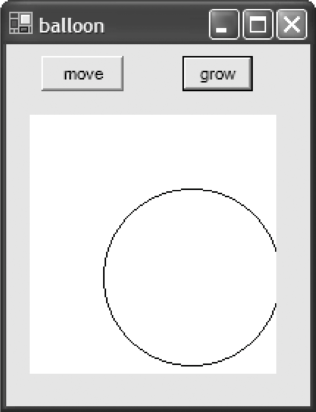
\includegraphics[width=5cm]{classes_balloon_screen}
					\caption{Screen layout for the balloon program.}
					\label{fig:classes_balloon_screen}
				\end{figure}

		We will construct this program from two objects and therefore two classes:
		\begin{itemize}
			\item Class \keyword{Balloon} represents the balloon. We can foresee that it will provide methods named \keyword{Move} and \keyword{ChangeSize} – with obvious meanings.
      \item Class \keyword{Form1} handles the GUI for the program. It uses class \keyword{Balloon} as necessary.
		\end{itemize}
		These are shown in the class diagram (\Vref{fig:classes_design}). A class diagram shows each class represented by a rectangle. Any connections between classes are shown as a line joining the two. In this case the relationship is shown as an annotation above the line.
		
		We will complete class \keyword{Form1} and then we will write class \keyword{Balloon}.

			\begin{figure}[th]
			\centering
				\begin{tikzpicture}[node distance=1.5cm]
					\node (Form1) [class] {Form1};
					\node (Balloon) [class, right = of Form1] {Balloon};
					
					\draw (Form1) -- node[above] {uses} (Balloon);
			\end{tikzpicture}
			\caption{Class diagram showing the two classes in the balloon program.}
			\label{fig:classes_design}
	 	\end{figure}


		At the head of the class \keyword{Form1}, we declare instance variables as usual, including a variable named \keyword{myBalloon}:
		\begin{lstlisting}
Private myBalloon As Balloon
Private drawArea As Graphics
		\end{lstlisting}
		Within \keyword{Sub New} we perform any necessary initialization, including creating a new instance of the class \keyword{Balloon}. This is the crucial step where we create an object from our own class.
		\begin{lstlisting}
myBalloon = New Balloon()
drawArea = PictureBox1.CreateGraphics()
		\end{lstlisting}
		Now the code to respond to button-click events:
		\begin{lstlisting}
Private Sub MoveButton_Click(sender As System.Object,
	e As System.EventArgs)
	Handles MoveButton.Click
	myBalloon.MoveRight(20)
	drawArea.Clear(Color.White)
	myBalloon.Display(drawArea)
End Sub
Private Sub GrowButton_Click(sender As System.Object,
		e As System.EventArgs)
		Handles GrowButton.Click
	myBalloon.ChangeSize(20)
	drawArea.Clear(Color.White)
	myBalloon.Display(drawArea)
End Sub
		\end{lstlisting}
		This concludes the coding for the class \keyword{Form1}. Writing this code helps us to clarify how a balloon object will be used, enabling us to see what methods and properties need to be provided by class \keyword{Balloon}, as well as the nature of any parameters. This leads us to write the code for class \keyword{Balloon}:
		\begin{lstlisting}
Public Class Balloon
	Private x As Integer = 50
	Private y As Integer = 50
	Private diameter As Integer = 20
	Dim myPen As Pen = New Pen(Color.Black)
	Public Sub MoveRight(xStep As Integer)
		x = x + xStep
	End Sub
	Public Sub ChangeSize(change As Integer)
		diameter = diameter + change
	End Sub
	Public Sub Display(drawArea As Graphics)
		drawArea.DrawEllipse(myPen, x, y, diameter, diameter)
	End Sub
End Class
		\end{lstlisting}
		The heading of a class description starts with the keywords \keyword{Public} and \keyword{Class}, and gives the class name. The complete description is terminated with an \keyword{End Class} statement. The VB convention is that names of classes start with a capital letter. The body of a class consists of declarations of variables, methods and properties. Note how the readability of the class is enhanced using blank lines and indentation. In the next few sections of this chapter we will go on to look in detail at each of the ingredients in the above class description for balloons.
		
		The overall structure of a class is:
		\begin{lstlisting}
Public Class Balloon
' variables
' methods
' properties
End Class
		\end{lstlisting}
		Where are classes held? One approach is to write all the classes and place them in a single file, but a better approach is to place different classes in different files. The IDE helps by providing a facility to do this. The steps are:
		\begin{enumerate}
			\item	Choose \ui{Add Class} from the \ui{Project} menu. A window appears.
			\item	Select \ui{Class} from the list of templates.
			\item	Type in the name of the file to hold the class (usually the name of the class with the extension \keyword{.vb}).
			\item	Click on \ui{Add}.
		\end{enumerate}
		This creates a distinct file to hold the code for the class. The file is part of the project for the program and it is automatically compiled and linked when the program is run.


	\section{Private variables}
		A balloon has data associated with it – its size (diameter) and its position (as $x$ and $y$ coordinates). A balloon object must remember these values. This data is held in variables that are described like this:
		\begin{lstlisting}
Private diameter As Integer
Private x, y As Integer
		\end{lstlisting}
		The variables \keyword{diameter}, \keyword{x} and \keyword{y} are declared at the top of the class. They can be accessed by any of the statements in the class. They are called \emph{class-level variables} or \emph{instance variables}.
		
		As we saw in \Cref{ch:objects}, you will see that the word normally used to introduce variables – \keyword{Dim} – has been replaced by the word \keyword{Private}. Class-level variables are almost always declared as \keyword{Private}. Although we \emph{could} describe these variables as \keyword{Public}, this is regarded as bad practice. Instead we keep them as \keyword{Private}, and use properties or methods to access their values, as we shall see.

		\begin{stqb}
			\begin{STQ}
				\item Extend the balloon object so that it has a variable that describes the colour of the balloon.
			\end{STQ}
		\end{stqb}

	\section{Public methods}
		Some features of an object need to be publicly available to other pieces of program. This includes those methods which, after all, have been designed for the use of others. As we have seen, a balloon has actions associated with it – for example, to change its size. These actions are written as methods. Changing the size is accomplished by:
		\begin{lstlisting}
Public Sub ChangeSize(change As Integer)
   diameter = diameter + change
End Sub
		\end{lstlisting}
		To signify that it is publicly available, we precede the method header with the VB word \keyword{Public}. Next we write the method to move a balloon:
		\begin{lstlisting}
Public Sub MoveRight(xStep As Integer)
	x = x + xStep
End Sub
		\end{lstlisting}
		To complete the class we provide an additional method for a balloon to display itself when requested to do so.
		
		We have now distinguished clearly between those items that we are making publicly available and those that are private. This is an important ingredient of the philosophy of OOP. Data (variables) and actions (methods) are bundled up together, but in such a way as to hide some of the information from the outside world. Normally it is the data that is hidden away from the rest of the world. This is termed \emph{encapsulation} or \emph{information hiding}.

		\begin{stqb}*
			\begin{STQ}
				\item Write a method that moves a balloon upwards by an amount given as the parameter. Name the method MoveUp.
				\item Write a method that an enables the colour of a balloon to be changed.
				\item Rewrite method Display so that it displays a coloured balloon.
			\end{STQ}
		\end{stqb}


		\begin{figure}[bth]
			\centering
			\begin{minipage}[t]{.45\textwidth}
			  \centering
				\begin{tikzpicture}[shorten >=1pt,auto,node distance= 1cm, scale = 0.8, transform shape]

					\begin{pgfonlayer}{main}
						\node[draw,align=center, fill=white] (class-var)  {class-level\\variables};
						\node[draw,align=center,below = of class-var] (public-method)  {\keyword{Public} MethodM\\lines of code};
						\node[draw,align=center, below= of public-method] (property)  {\keyword{Public} PropertyP\\lines of code};
						\node[draw,align=center, below= of property] (private-method)  {\keyword{Private} methods\\lines of code};
					\end{pgfonlayer}

			    \begin{pgfonlayer}{background}
    		    % Following lines added
						\node (X) [fit= (class-var) (public-method) (property) (private-method), inner sep=1cm, draw=black, ultra thick] {};
	    		\end{pgfonlayer}
				\end{tikzpicture}			
				\caption{Structure of an object or class as seen by the programmer who writes it.}
				\label{fig:classes_object_view_programmer}
		\end{minipage}\hfill%5 create void between figures
			\begin{minipage}[t]{.45\textwidth}
			  \centering
				\begin{tikzpicture}[shorten >=1pt,auto,node distance= 1cm, scale = 0.8, transform shape]
					\begin{pgfonlayer}{main}
						\node[draw,align=center] (class-var)  {class-level\\variables};
						\node[draw,align=center,below = of class-var,fill=white] (public-method)  {\keyword{Public} MethodM\\lines of code};
						\node[draw,align=center, below= of public-method, fill= white] (property)  {\keyword{Public} PropertyP\\lines of code};
						\node[draw,align=center, below= of property] (private-method)  {\keyword{Private} methods\\lines of code};
					\end{pgfonlayer}

			    \begin{pgfonlayer}{background}
  	  		    % Following lines added
						\node (X) [draw=black, fit= (class-var) (public-method) (property) (private-method), inner sep=1cm, ultra thick, fill=black] {};
    			\end{pgfonlayer}
				\end{tikzpicture}					
				\caption{Structure of an object or class as seen by its users.}
				\label{fig:classes_object_view_user}
			\end{minipage}
		\end{figure}



		A class or object has the general structure shown in \Vref{fig:classes_object_view_programmer}. This is the view as seen by the programmer who writes it – it consists of variables, properties and methods. The view of an object as seen by its users is shown in \Vref{fig:classes_object_view_user}. The view to its users, to whom it is providing a service, is very different. Only the public items (usually methods and properties) are visible – everything else is hidden within an impenetrable box.

		
	\section{Properties}
		We have seen that it is very bad practice to make \keyword{Public} any of the instance variables of a class. The way to give users convenient but controlled access to the data associated with an object is to use properties. We have already used properties of components of the toolkit. For example, we can write statements to access the values of the properties of a text box:
		\begin{lstlisting}
name = TextBox1.Text
TextBox1.Visible = False
		\end{lstlisting}
		These are examples of accessing data that is part of an object. Notice that there are two distinct kinds of access:
		\begin{itemize}
			\item Reading a value – this is called \emph{get} access (for example extracting the text from a text box using the \keyword{Text} property).
			\item Writing the value – this is called \emph{set} access (for example changing the \keyword{Visible} property of a text box).
		\end{itemize}
		We will now explore how to provide these kinds of access to data. For example, suppose we want to allow a user of a balloon object to refer to (get) the $x$ coordinate of the balloon. This is held in the variable named \keyword{X} at the top of the class. As a user of a balloon object, \keyword{myBalloon}, we want to be able to extract and use the value, as in:
		\begin{lstlisting}
TextBox1.Text = CStr(myBalloon.XCoord)
		\end{lstlisting}
		Suppose also that we want the user to be able to change (set) the value of the $x$ coordinate with a statement such as:
		\begin{lstlisting}
myBalloon.XCoord = 56
		\end{lstlisting}
		The way to provide these facilities is to write a property. Here is the revised class that includes the property code:
		\begin{lstlisting}
Public Class BalloonWithProperties
	Private x As Integer = 50
	Private y As Integer = 50
	Private diameter As Integer = 20
	Private myPen As Pen = New Pen(Color.Black)
	Public Sub MoveRight(xStep As Integer)
		x = x + xStep
	End Sub
	Public Sub ChangeSize(change As Integer)
		diameter = diameter + change
	End Sub
	Public Sub Display(drawArea As Graphics)
		drawArea.DrawEllipse(myPen, x, y, diameter, diameter)
	End Sub
	Public Property XCoord() As Integer
		Get
			Return x
		End Get
		Set(value As Integer)
			x = value
		End Set
	End Property
End Class
		\end{lstlisting}
		The name of the property (\keyword{XCoord} in this example) follows the keyword \keyword{Property} in the header. The complete declaration ends with the \keyword{End Property} statement.
		
		The description consists of two complementary components – one has \keyword{Get} as the heading and the other has \keyword{Set} as the heading. Each component ends with its respective \keyword{End Get} or \keyword{End Set}. The \keyword{Get} part is just like a function – it returns the desired value. The \keyword{Set} part is just like a method – it assigns the value of the parameter (named \keyword{value} in this example) as shown.
		
		We can now use these properties in the program that uses this class. We enhance it to provide a button to display the value of the $x$ coordinate in a text box. \Vref{fig:classes_balloon_properties_screen} shows the screen.
		
		\begin{figure}[bth]
			\centering
			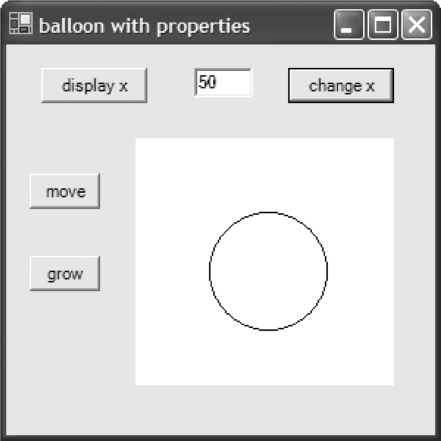
\includegraphics[width=7cm]{classes_balloon_properties_screen}
			\caption{Balloon program using properties.}
			\label{fig:classes_balloon_properties_screen}
		\end{figure}


		The code that responds to a click on the button to display the $x$ coordinate is given below. It uses the \keyword{Get} property that we have just seen:
		\begin{lstlisting}
Private Sub DisplayXButton_Click(
		sender As System.Object,
		e As System.EventArgs)
		Handles DisplayXButton.Click
	TextBox1.Text = CStr(myBalloon.XCoord)
End Sub
		\end{lstlisting}
		The program also provides a button to change the $x$ coordinate (entered in the text box). It uses the \keyword{Set} property that we have just seen. The code that responds to a click on this button is:
		\begin{lstlisting}
Private Sub ChangeXButton_Click(
		sender As System.Object,
		e As System.EventArgs)
		Handles ChangeXButton.Click
	myBalloon.XCoord = CInt(TextBox1.Text)
	myBalloon.Display(drawArea)
End Sub
		\end{lstlisting}
		If we only need a way of viewing a property (but not changing its value), we write the property declaration with the prefix \keyword{ReadOnly} like this:
		\begin{lstlisting}
Public ReadOnly Property XCoord() As Integer
	Get
		Return x
	End Get
End Property
		\end{lstlisting}
		If, on the other hand, we need to change a value, but do not need the facility to view it, we write:
		\begin{lstlisting}
Public WriteOnly Property XCoord() As Integer
	Set(value As Integer)
		x = value
	End Set
End Property
		\end{lstlisting}
		When you see properties for the first time, you may be tempted to wonder why such a long-winded mechanism is needed. Surely it would be easier simply to declare the value \keyword{x} as \keyword{Public}? Then the user of the object could simply refer to the value as \keyword{myBalloon.x}. There are several reasons:
		\begin{itemize}
      \item The class can hide the internal representation of the data from the users, while still maintaining the external interface. For example, the author of the balloon class might choose to hold the coordinates of the centre point of a balloon, but provide users with the coordinates of the top left of an enclosing square.
			\item The author of the class can decide to restrict access to data. For example restrict the $x$ coordinate to read-only (\keyword{Get}) access, while disallowing write (\keyword{Set}) access.
      \item The class can validate or screen the values used. For example, ignore negative values for a coordinate.
		\end{itemize}

		\begin{stqb}
			\begin{STQ}
				\item Write properties to allow a user \keyword{Set} and \keyword{Get} access to the $y$ coordinate of a balloon.
			\end{STQ}
		\end{stqb}


	\section{Method or property?}
		Methods and properties both provide mechanisms for accessing an object. So how do we choose which to use? The answer is that we use methods when we want an object to carry out some action. (A method usually has a name that is a verb.) We use properties when we want to refer to some information associated with an object. (A property usually has a name that is a noun.)

		We can see this in the library classes. For example, a text box has methods \keyword{Clear} and \keyword{AppendText} to carry out actions. It has properties \keyword{Text} and \keyword{Visible} to refer to the state of the object.

		Examples of methods associated with a balloon, discussed above, are: \keyword{Display}, \keyword{MoveUp}, \keyword{MoveDown}, \keyword{MoveLeft}, \keyword{MoveRight}, \keyword{Shrink} and \keyword{Grow}.

		Examples of balloon properties are: \keyword{XCoord}, \keyword{YCoord}, \keyword{Diameter}, \keyword{Colour} and \keyword{Visible}.

		Sometimes there is a choice over whether to make something a property or a method, and the choice is a matter of style. For example, to change the colour of a component we could have a method \keyword{ChangeColour}; alternatively we could have a property \keyword{Colour}.

		\begin{stqb}
			\begin{STQ}
				\item In designing a class \keyword{Account} to represent a bank account, which of the following should be methods and which should be properties?
					\begin{lstlisting}
CreditAccount, DebitAccount, CurrentBalance,
CalculateInterest, Name
					\end{lstlisting}
			\end{STQ}
		\end{stqb}


	\section{Constructors}
		When a balloon object is created, the position and size of the balloon need to be given some values. This is called initializing the variables. There are two ways to do the initialization of variables. One way is to do the initialization as part of the declaration of the class-level variables:
		\begin{lstlisting}
Private x As Integer = 50
Private y As Integer = 50
Private diameter As Integer = 20
		\end{lstlisting}
		Another way to initialize an object is to write a special method to do the initialization. This method is named a \emph{constructor method} or simply a \emph{constructor} (because it is involved in the construction of the object). This method always has the special name \keyword{New}. It has no return value, but it can have parameters. Here is a constructor method for the \keyword{Balloon} class:
		\begin{lstlisting}
Public Sub New(initialX As Integer,
		initialY As Integer,
		initialDiameter As Integer)
	x = initialX
	y = initialY
	diameter = initialDiameter
End Sub
		\end{lstlisting}
		This method assigns the values of the parameters (the size and position) to the appropriate variables within the object. A constructor method such as this is written at the top of the class, after the declarations of the class-level variables.
		
		The above constructor method would be used as shown by this example:
		\begin{lstlisting}
Dim myBalloon As Balloon = New Balloon(10, 10, 50)
		\end{lstlisting}
		If a variable is not explicitly initialized by the programmer, the VB system gives every variable a default value. This is zero for any numbers, \keyword{False} for a \keyword{Boolean}, “ ” (an empty string) for a \keyword{String} and the value \keyword{Nothing} for any object. It is regarded as bad practice to rely on this method of initialization of variables. Instead, it is better to do it explicitly either when the item is declared or by a statement in a constructor.
		
		Other actions that a constructor method might take include creating any objects that the object uses or opening a file that the object uses.
		
		If a class does not have an explicit constructor, then it is assumed to have a single constructor with zero parameters, known as the default constructor.


	\section{Multiple constructors}
		A class can have none, one or several constructor methods. If a class has one or more constructors, they will normally involve parameters and must be called with the appropriate parameters. For example, in the \keyword{Balloon} class, we can write the two constructors:
		\begin{lstlisting}
Public Sub New(initialX As Integer,
		initialY As Integer,
		initialDiameter As Integer)
	x = initialX
	y = initialY
	diameter = initialDiameter
End Sub
Public Sub New(initialX As Integer,
		initialY As Integer)
	x = initialX
	y = initialY
	diameter = 20
End Sub
		\end{lstlisting}
		which would allow us to create balloon objects in either of the following ways:
		\begin{lstlisting}
Dim balloon1 As Balloon = New Balloon(10, 10, 50)
Dim balloon2 As Balloon = New Balloon(10, 10)
		\end{lstlisting}
		but not allow:
		\begin{lstlisting}
Dim balloon3 As Balloon = New Balloon()
		\end{lstlisting}
		So if you write several constructors, but you still need a constructor with zero parameters, you must explicitly write it, for example:
		\begin{lstlisting}
Public Sub New()
End Sub
		\end{lstlisting}
		We have now written three constructors for the class \keyword{Balloon}, and here is how they might be used to create three different objects from the same class:
		\begin{lstlisting}
Dim balloon1 As Balloon = New Balloon()
Dim balloon2 As Balloon = New Balloon(10, 10, 50)
Dim balloon3 As Balloon = New Balloon(10, 10)
		\end{lstlisting}

		\begin{stqb}
			\begin{STQ}
				\item Write a constructor method to create a new balloon, specifying only the diameter.
			\end{STQ}
		\end{stqb}


	\section{Private methods}
	The whole purpose of writing a class is to allow the creation of objects that present useful facilities to other objects. These facilities are the \keyword{Public} methods and properties that the object offers. But often a class has methods that do not need to be made public and, indeed, all the methods in the programs given earlier in this book are \keyword{Private}. In the \keyword{Balloon} class, suppose we wanted to supply a method that allowed another object to find out the area of a balloon. This would be provided as a \keyword{Public} method and let us name this method \keyword{Area}. However, we might decide that the detailed calculation of the area is a little complicated and therefore should be packaged up within another \keyword{Private} method named \keyword{CalcArea} that \keyword{Area} calls when it needs to. We have created a \keyword{Private} method that acts in support of the public methods in the class:
		\begin{lstlisting}
Private Function CalcArea() As Double
	Dim radius As Double	
	radius = diameter / 2.0
	Return 3.142 * radius * radius
End Function
		\end{lstlisting}
		To call a method from within the object, you do it like this:
		\begin{lstlisting}
Dim area As Double
area = CalcArea()
		\end{lstlisting}
		giving the name of the method and any parameters as usual. If this method was called by another object, it would need to be prefixed by the name of an object. But because it is called by a method within the same object, the object is implicit. If we really want to emphasize which object is being used, we could write the following equivalent code:
		\begin{lstlisting}
area = Me.CalcArea()
		\end{lstlisting}
		using the keyword \keyword{Me} that means the current object.
		
		Depending on its size and complexity a class might have a number of private methods. Their purpose is to clarify and simplify the class.


	\section{Operations on objects}
		Many of the variables that are used in VB programs are true objects, but some variables are not. Variables declared as \keyword{Integer}, \keyword{Boolean} and \keyword{Double} are not objects, but are called \emph{primitive types}. When you declare a primitive variable, it is immediately usable. For example:
		\begin{lstlisting}
Dim number As Integer
		\end{lstlisting}
		both declares the variable \keyword{number} and creates it. By contrast, the creation of an object has to be done explicitly either using \keyword{New} (or graphically by dragging the class from the toolbox). For example:
		\begin{lstlisting}
Dim balloon1 As Balloon = New Balloon(10, 20, 50)
		\end{lstlisting}
		So variables in VB are either:
		\begin{itemize}
			\item primitive types such as \keyword{Integer}, \keyword{Boolean} and \keyword{Double}; these are not objects, or
      \item objects created from classes, either visually or by using \keyword{New}.
		\end{itemize}
		Primitive variables come ready-made with a whole collection of things you can do with them. For example, with variables of type \keyword{Integer} you can:
		\begin{itemize}
      \item declare variables;
      \item assign values using =;
      \item carry out arithmetic;
      \item compare using =, <, etc.;
      \item use as a parameter or as a return value.
		\end{itemize}
		You cannot necessarily do all these things with objects. Many things that a VB program uses are objects but, as we have seen, not everything is an object. And it is tempting to assume that it is possible to use all these operations with any object but this is not so. What can you do with an object? The answer is that when you write a class, you define the collection of operations that can be performed on objects of that type. With the \keyword{Balloon} class, for example, we have defined the operations \keyword{ChangeSize}, \keyword{Move} and \keyword{Display}. The programmer should not assume that you can do anything else to a balloon. However, you can confidently assume that for every object you can:
		\begin{itemize}
      \item create it;
      \item use it as a parameter and as a return value;
      \item assign it to a variable of the same class using =;
      \item use the methods and properties that are provided as part of its class.
		\end{itemize}

		\begin{stqb}
			\begin{STQ}
				\item Write down a list of operations that are possible with an object of the class \keyword{Balloon} and give examples of using them.
			\end{STQ}
		\end{stqb}


	\section{Object destruction}
		We have seen how objects are created, using the powerful word \keyword{New}. How do they die? One obvious and certain situation is when the program ceases to run. They can also die when they cease to be used by the program. For example, if we do this to create a new object:
		\begin{lstlisting}
Dim myBalloon As Balloon
myBalloon = New Balloon(20, 100, 100)
		\end{lstlisting}
		and then:
		\begin{lstlisting}
myBalloon = New Balloon(40, 200, 200)
		\end{lstlisting}
		what happens is that the first object created with \keyword{New} lived a brief life. It died when the program no longer had any knowledge of it and its value was usurped by the newer object. When an object is destroyed, the memory that was used to store the values of its variables and any other resources is reclaimed for other uses by the run-time system. This is termed \emph{garbage} collection. In VB, garbage collection is automatic. (In some other languages it is not and the programmer has to keep track of objects that are no longer needed.)
		
		Finally, we can destroy an object by assigning the value \keyword{Nothing} to it, for example:
		\begin{lstlisting}
myBalloon = Nothing
		\end{lstlisting}
		The word \keyword{Nothing} is a special VB word that describes a non-existent (un-instantiated) object.


	\section{Shared methods and properties}
	Some methods do not need an object to work on. An example is the mathematical square root function. Mathematical methods such as square root (\keyword{Sqrt}) and sine of an angle (\keyword{Sin}) are provided within a library class named \keyword{Math}. In a program we write statements such as:
		\begin{lstlisting}
Dim x, y As Double
x = Math.Sqrt(y)
		\end{lstlisting}
		In this statement there are two \keyword{Double} variables, \keyword{x} and \keyword{y}, but no objects. Note that \keyword{Math} is the name of a class, not an object. The square root method \keyword{Sqrt} acts on its parameter, y. The question is: if \keyword{Sqrt} is not a method of some object, what is it? The answer is that methods like this are part of a class, but they are described as \keyword{Shared}. When you use one of these methods, its name must be preceded with the name of its class.
		
		The class \keyword{Math} has the following structure, in which the methods are labelled as \keyword{Shared}:
		\begin{lstlisting}
Public Class Math
	Public Shared Function Sqrt(x As Double) As Double
		' body of Sqrt
	End Function
	Public Shared Function Sin(x As Double) As Double
		' body of Sin
	End Function
End Class
		\end{lstlisting}
		Other examples of \keyword{Shared} methods are \keyword{CInt} and \keyword{CStr}. An example of a \keyword{Shared} property is to be seen in the library class \keyword{Color}. The various colours are available for use by other classes as \keyword{Color.White}, \keyword{Color.Black}, etc. Other \keyword{Shared} properties are \keyword{NewLine} and \keyword{Tab}.
		
		What is the point of \keyword{Shared} methods? In OOP, everything is written as a part of a class; nothing exists other than classes. If we think about the \keyword{Balloon} class, it contains \keyword{Private} variables such as \keyword{x} and \keyword{y}that record the state of an object. But some methods, such as \keyword{Sqrt}, do not involve a state. So free-standing methods such as \keyword{Sqrt} which are not obviously part of some class, have to obey the central rule of OOP – they have to be a part of some class. Hence the reason for \keyword{Shared} methods. It is common for programmers to make use of the library \keyword{Shared} methods and properties but it is rare for novice programmers to write them.
		
		Incidentally, there is a more concise way of calling a shared method such as \keyword{Sqrt}, provided that a suitable \keyword{Imports} statement appears at the head of the program. So, once we have written this at the top of the program:
		\begin{lstlisting}
Imports System.Math
We can subsequently write the more concise:
x = Sqrt(y)
		\end{lstlisting}

		\begin{stqb}
			\begin{STQ}
				\item The \keyword{Shared} method \keyword{Max} within the class \keyword{Math} finds the maximum of its two \keyword{Integer} parameters. Write a sample call on \keyword{Max}.
			\end{STQ}
		\end{stqb}


	\section{Programming principles}
	Object-oriented programming is about constructing programs from objects. An \emph{object} is a combination of some data (variables) and some actions (methods) that performs some useful role in a program. The programmer designs an object so that the data and the actions are closely related, rather than being randomly collected together.
		
	In VB, as in most OOP languages, it is not possible to write instructions that describe an object directly. Instead the language makes the programmer define all objects of the same class. For example, if we need a button object, we go to the tool bar and select the Button class. We drag an instance of this class and place it on the form. If we need a second button, we create a second instance of this same class. The description of the structure of all possible buttons is called a \emph{class}. A class is the template or the master plan to make any number of them; a class is a generalization of an object.
		
		The idea of classes is a common idea in most design activity. It is usual before actually constructing anything to create a design for the object. This is true in automobile design, architecture, construction – even in fine art. Some kind of a plan is drafted, often on paper, sometimes on a computer. Sometimes it is called a blueprint. Such a design specifies the desired object completely, so that if the designer gets run over by a bus, someone else can carry out the construction of the object. Once designed, any number of identical objects can be constructed – think of cars, books or computers. So the design specifies the composition of one or any number of objects. The same is true in OOP – a class is the plan for any number of identical objects. Once we have specified a class, we can construct any number of objects with the same behaviour.
		
		Looking at the button again, what we have is the description of what each and every button object will look like. Buttons only differ in their individual properties, such as their positions on the form. So in OOP, a class is the specification for any number of objects that are the same. Once a class has been described, a particular object is constructed by creating an \emph{instance} of the class. It's a bit like saying we have had an instance of flu in the house. Or, this Model T Ford is an instance of the Model T Ford design. Your own bank account is an instance of the bank account class.
		
		An object is a logical bundling together of variables, methods and properties. It forms a self-contained module that can be easily used and understood. The principle of information hiding or encapsulation means that users of an object have a restricted view of an object. An object provides a set of services as \keyword{Public} methods and properties that others can use. The remainder of the object, its variables and the instructions that implement the methods are hidden from view. This enhances abstraction and modularity.
		
		In programming, the term \emph{accessibility} (sometimes called \emph{scope rules} or \emph{visibility}) means the rules for accessing variables and methods. For humans, accessibility rules are like the rule that in Australia you must drive on the left, or the rule that you should only enter someone's home via the front door. In a program, rules like these are rigidly enforced by the compiler, to prevent deliberate or erroneous access to protected information. Accessibility rules constrain the programmer, but help the programmer to organize a program in a clear and logical manner. The accessibility rules associated with classes and methods allow the programmer to encapsulate variables and methods in a convenient manner.
		
		The programmer can describe each variable, method and property as either \keyword{Public} or \keyword{Private}. Within a class, any instruction anywhere in the class can call any method, \keyword{Public} or \keyword{Private}. Also any instruction can refer to any variable. The exception is that local variables, those declared within a method, are only accessible by instructions within the method.
		
		When one class refers to another, only those methods, properties and variables labelled as \keyword{Public} are accessible from outside a class. All others are inaccessible. It is good design practice to minimize the number of methods and properties that are \keyword{Public}, restricting them so as to offer only the services of the class. It is also good practice never (or very rarely) to make variables \keyword{Public}. If a variable needs to be inspected or changed, a method or property should be provided to do the job.
		
		In summary, a variable, method or property within a class can be described as either:
		\begin{itemize}
      \item \keyword{Public} – accessible from anywhere (from within the class or from any other class); or
      \item \keyword{Private} – accessible only from within the class.
		\end{itemize}

		In computer science a class is sometimes called an \emph{abstract data type}(ADT). A data type is a kind of variable, like an \keyword{Integer}, a \keyword{Double} or a \keyword{Boolean}. These primitive types are types built into the VB language and are immediately available for use. Associated with each of these types is a set of operations. For example, with an \keyword{Integer} we can do assignment, addition, subtraction and so on. The \keyword{Balloon} class described above is an example of an ADT. It defines some data (variables), together with a collection of operations (methods) and properties that can carry out operations on the data. The class presents an abstraction of a balloon; the concrete details of the implementation are hidden.
		
		Look at the code that is created when you open a new VB windows application within the Integrated Development Environment. You will see the following code is automatically created:
		\begin{lstlisting}
Public Class Form1
		\end{lstlisting}
		As you can see this is a description of a class called \keyword{Form1}, because like everything else a form is a class. When the run-time system starts this program it implicitly carries out a
		\begin{lstlisting}
Dim myForm As Form1 = New Form1()
		\end{lstlisting}
		statement to create an object from this class. You will not see this instruction in any program because it is hidden within the run-time system. Thus the run-time system acts as a god, creating the first object in the world. This object itself goes on to create other objects, such as buttons.


	\section{Programming pitfalls}
		\begin{itemize}
      \item Novices sometimes want to code an object straight away. You can't – instead you have to declare a class and then create an instance of the class.
      \item \keyword{New} is used for two purposes – the word used to create an object and the name of a constructor method.
      \item Do not forget to initialize instance variables. Explicitly initialize them by means of a constructor method or as a part of the declaration itself and do not rely on VB's default initialization.
		\end{itemize}
		If you declare:
		\begin{lstlisting}
Dim redBalloon As Balloon
		\end{lstlisting}
		and then perform:
		\begin{lstlisting}
redBalloon.Display()
		\end{lstlisting}
		your program will terminate with an error message that says there is a \keyword{Nothing} pointer exception. This is because you have declared an object but not created it (with \keyword{New}). The object \keyword{redBalloon} does not exist. More accurately, it has the value \keyword{Nothing} – which amounts to the same thing. In most elementary programming you do not make use of \keyword{Nothing} – except if you inadvertently forget to use \keyword{New}.


	\section{Grammar spot}
		\begin{itemize}
      \item A class has the structure:
				\begin{lstlisting}
Public Class ClassName
	‘ declarations of variables
	‘ declarations of methods and properties
End Class
				\end{lstlisting}
      \item Variables, methods and properties can be either described as \keyword{Public} or \keyword{Private}.
      \item One or more of the methods in a class can have the name \keyword{New}. One of these constructor methods may be called (with appropriate parameters) to initialize the object when it is created.
      \item The declaration of a public method has the structure:
				\begin{lstlisting}
Public Sub MethodName(parameters)
	' body
End Sub
				\end{lstlisting}
      \item The declaration of a property has the structure:
				\begin{lstlisting}
Public Property Name() As Integer
	Get
		' statements to return a value
	End Get
	Set (value As Integer)
		' statements to assign value to some variable
	End Set
End Property
				\end{lstlisting}
			\item A \keyword{Property} can be declared \keyword{ReadOnly} (with no \keyword{Set} part) or \keyword{WriteOnly} (with no \keyword{Get} part).
			\item A shared method or property is prefixed by the word \keyword{Shared} in its header:
      \item To call a shared method of a class:
				\begin{lstlisting}
ClassName.MethodName(parameters)
				\end{lstlisting}
		\end{itemize}


	\section{New language elements}
		\begin{itemize}
			\item \keyword{Class}: appears in the heading of the description of a class.
			\item \keyword{Public}: the description of a variable, method or property that is accessible from anywhere.
			\item \keyword{Private}: the description of a variable, method or property that is only accessible from within the class.
			\item \keyword{New}: used to create a new instance of a class (a new object).
			\item \keyword{New}: the name of a constructor method of a class.
			\item \keyword{Property}: introduces a property declaration.
			\item \keyword{Set}: introduces the part of a property declaration that changes the value of the property.
			\item \keyword{Get}: introduces the part of a property declaration that returns a value.
			\item \keyword{ReadOnly}: prefaces a property that can only access (but not change) the value of the property.
			\item \keyword{WriteOnly}: prefaces a property that can only change the value of the property.
			\item \keyword{Me}: the name of the current object.
			\item \keyword{Nothing}: the name of an object that does not exist.
			\item \keyword{Shared}: the description attached to a variable, property or method that belongs to a class as a whole, not to any instance created as an object from the class.
		\end{itemize}


	\section{Summary}
		\begin{itemize}
      \item An object is a collection of data and the associated actions, methods and properties, that can act upon the data. VB programs are constructed as a collection of objects.
      \item One particular method, named \keyword{New}, carries out the initialization of a newly created object. This is termed the constructor method.
      \item Items in a class can be declared to be \keyword{Private} or \keyword{Public}. A \keyword{Private} item can only be referred to from within the class. A \keyword{Public} item can be referred to by anything (inside or outside the class). In designing a VB program, \keyword{Public} items are normally kept to a minimum so as to enhance information hiding. 
				
				In particular, data items are usually kept private.
			\item The description \keyword{Shared} means that the variable, property or method belongs to the class and not to particular objects. A Shared method can be called directly, without any need for instantiating an instance of the class with \keyword{New}. A \keyword{Shared} method or property is useful when a method does not need to be associated with a particular object, or for carrying out actions for the class as a whole.
		\end{itemize}


	\section{Exercises}
		\begin{EXE}
			\item \name{Balloons} Add to the class \keyword{Balloon} some additional data, a \keyword{String} that holds the name of the balloon and a variable that describes its colour. Add code to initialize these values using a constructor method and add the code to display them.
		Enhance the balloon program with buttons that move the balloon left, right, up and down.
			\item \name{Amplifier display} Some stereo amplifiers have a display that shows the volume being output. The display waxes and wanes according to the volume at any point in time. Some displays have indicators that show the maximum and minimum values that have been reached since the amplifier was switched on.
				
				Write a program that displays in text boxes the values of the maximum and minimum values that a track bar has been set to.
				
				Write the piece of program that remembers the values and compares them as a class. This class has a method \keyword{NewValue} and properties \keyword{LowestValue} and \keyword{HighestValue}.
			\item \name{Bank account} Write a program that simulates a bank account. A text box allows deposits (a positive number) to be made into the account and withdrawals (a negative number) to be made. The state of the account is continually displayed and, if the account goes into the red (negative balance), a suitable message is displayed. Create a class named Account to represent bank accounts. It has methods \keyword{Deposit} and \keyword{Withdraw}, and a property \keyword{Currentbalance}.
			\item \name{Scorekeeper} Design and write a class that acts as a scorekeeper for a computer game. It maintains a single integer, the score. It provides a method to initialize the score to zero, a method to increase the score, a method to decrease the score, and a method to return the score. Write instructions to create a single object and use it.
			\item \name{Dice} Design and write a class that acts as a die, which may be thrown to give a value 1 to 6. Initially write it so that it always gives the value 6. Write a program that creates a die object and uses it. The screen displays a button, which when pressed causes the die to be thrown and its value displayed.

				Then alter the die class so that it gives the value one higher than when it was last thrown, for example 4 when it was 3.

				Then alter it so that it uses the library random number generator.

				Some games like backgammon and Monopoly need two dice. Write VB statements to create two instances of the dice object, throw them and display the outcomes.
			\item \name{Random number generator} Write your own random number generator as a class that uses a formula to obtain the next pseudo-random number from the previous one. A random number program works by starting with some ‘seed' value. Thereafter the current random number is used as a basis for the next by performing some calculation on it which makes it into some other (apparently random) number. A good formula to use for integers is:
				\begin{lstlisting}
nextR = ((oldR * 25173) + 13849) Mod 65536
				\end{lstlisting}
				which produces numbers in the range 0 to 65535. The particular numbers in this formula have been shown to give good, random-like, results.
			\item \name{Complex numbers} Write a class called \keyword{Complex} to represent complex numbers (together with their operations). A complex number consists of two parts – a real part (a \keyword{Double}) and an imaginary part (a \keyword{Double}). The constructor method should create a new complex number, using the Double values provided as parameters, like this:
				\begin{lstlisting}
Dim c As Complex = New Complex(1.0, 2.0)
				\end{lstlisting}
				Write methods \keyword{GetReal} and \keyword{GetImaginary} to get the real part and the imaginary part of a complex number and which is used like this:
				\begin{lstlisting}
Dim x As Double = c.GetReal()
				\end{lstlisting}
				Write a method to add two complex numbers and return their sum. The real part is the sum of the two real parts. The imaginary part is the sum of the two imaginary parts. A call of the method looks like:
				\begin{lstlisting}
Dim c As Complex = c1.Sum(c2)
				\end{lstlisting}
				Write a method to calculate the product of two complex numbers. If one number has components $x_1$ and $y_1$ and the second number has components $x_2$ and $y_2$:
      \item the real part of the product $= x_1 × x_2 − y_1 × y_2$
      \item the imaginary part of the product $= x_1 × y_2 + x_2 × y_1$
		\end{EXE}

		\begin{stab}
			\begin{enumChapter}
				\item \ \begin{lstlisting}
Private myColor As Color
					\end{lstlisting}	
				\item \	\begin{lstlisting}
Public Sub MoveUp(amount As Integer)
	yCoord = yCoord – amount
End Sub
					\end{lstlisting}
				\item \ \begin{lstlisting}
Public Sub ChangeColor(newColor As Color)
	myColor = newColor
End Sub
					\end{lstlisting}
				\item \ \begin{lstlisting}
Public Sub Display(drawArea As Graphics)
	Dim myPen As Pen = New Pen(myColor)
	drawArea.DrawEllipse(myPen, x, y, diameter, diameter)
End Sub
					\end{lstlisting}
				\item \ \begin{lstlisting}
Public Property YCoord() As Integer
	Get
		Return y
	End Get
	Set(value As Integer)
		y = value
	End Set
End Property
					\end{lstlisting}
				\item	Methods: \keyword{CreditAccount}, \keyword{DebitAccount}, \keyword{CalculateInterest}
				
					Properties: \keyword{CurrentBalance}, \keyword{Name}
				\item \ \begin{lstlisting}
Public Sub New(initialDiameter As Integer)
	diameter = initialDiameter
End Sub
					\end{lstlisting}
				\item	Methods are: \keyword{ChangeColor}, \keyword{MoveUp}, \keyword{MoveRight}, \keyword{ChangeSize}, \keyword{Display}.
					
					Examples:
					\begin{lstlisting}
		myBalloon.ChangeColor(Color.Red)
		myBalloon.MoveUp(20)
		myBalloon.MoveRight(50)
		myBalloon.ChangeSize(10)
		myBalloon.Display(drawArea)
					\end{lstlisting}
					Properties are: \keyword{XCoord}, \keyword{YCoord}, \keyword{Diameter}
					
					Examples:
					\begin{lstlisting}
myBalloon.XCoord = 20
Dim y = myBalloon.YCoord
myBalloon.Diameter = 50
					\end{lstlisting}
					\item \
					\begin{lstlisting}
Dim x as Integer
x = Math.Max(7, 8)
					\end{lstlisting}
			\end{enumChapter}
		\end{stab}
